\documentclass{article}
\usepackage[english]{babel}
\usepackage[letterpaper,top=2cm,bottom=2cm,left=3cm,right=3cm,marginparwidth=1.75cm]{geometry}

\usepackage{amsmath}
\usepackage{graphicx}
% add graphics path
\graphicspath{{./graph/}}
\usepackage{indentfirst}
\usepackage{amsfonts}
\usepackage{caption}
\usepackage[colorlinks=true, allcolors=blue]{hyperref}

\usepackage{upgreek}

\title{Assignment 2}
\author{Shuhao Bian}

\begin{document}
\maketitle

\section{Problem 1}

% insert a pdf here
\begin{figure}[h!]
    \centering
    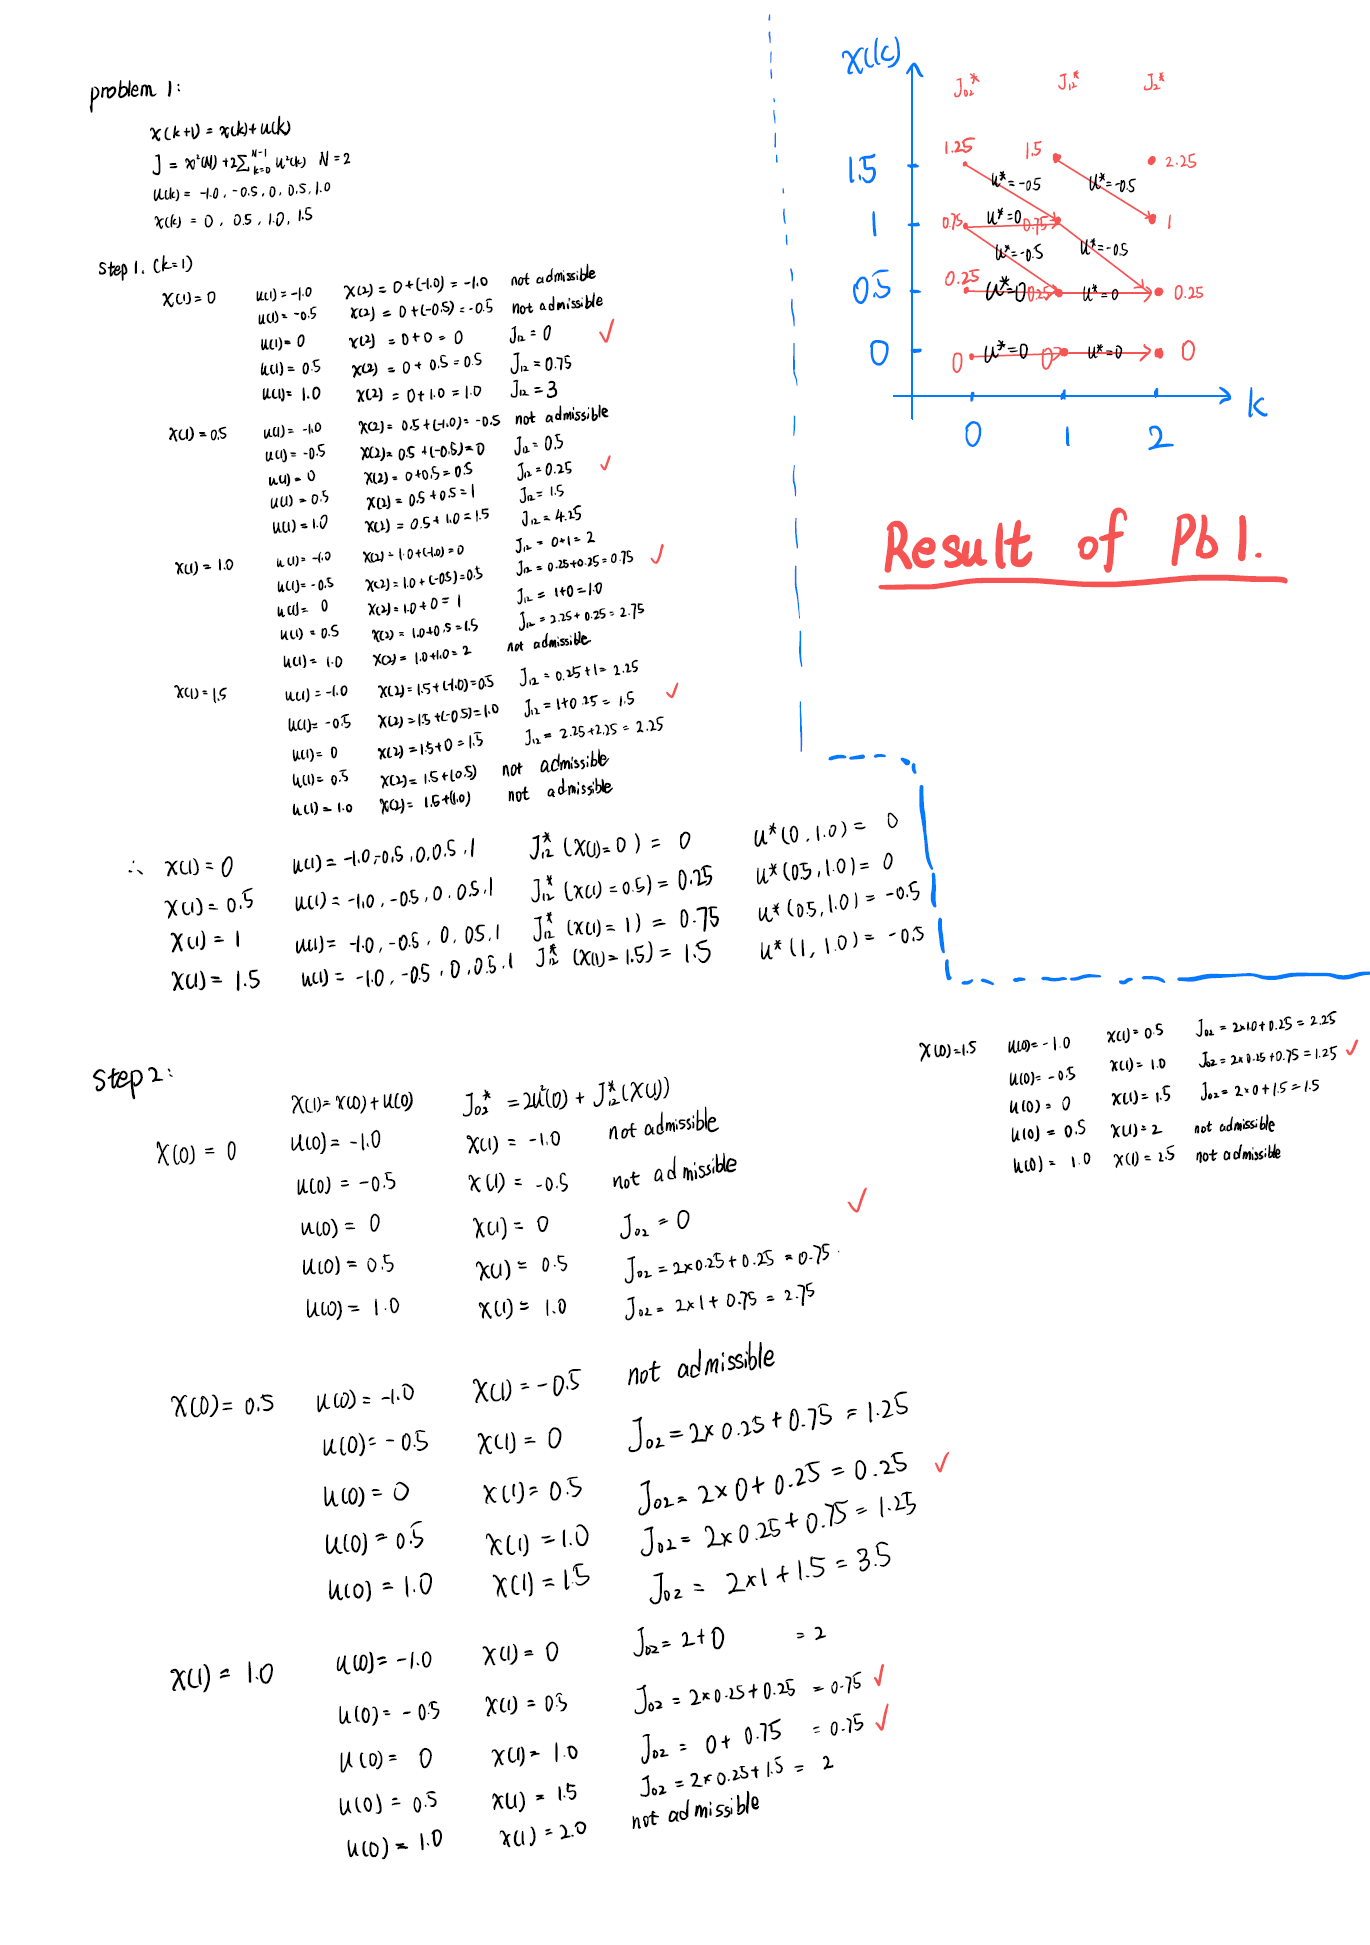
\includegraphics[width=0.7\textwidth]{graph 1.png}
    \caption{Graph 1}\label{fig:pb1graph1}
\end{figure}

According to the Figure \ref{fig:pb1graph1}, the best input is:
%itemize
\begin{itemize}
    \item $ x^*(0)=1\rightarrow x^*(1)=1\rightarrow x^*(2)=0.5, (u^*(1)=0, u^*(2)=-0.5)$
    \item $ x^*(0)=1\rightarrow x^*(1)=0.5\rightarrow x^*(2)=0.5, (u^*(1)=-0.5, u^*(2)=0)$
\end{itemize}
\newpage
\section{Problem 2}
\subsection{No constrants input, $T_s=0.1s$}

\begin{figure}[h!]
    \centering
    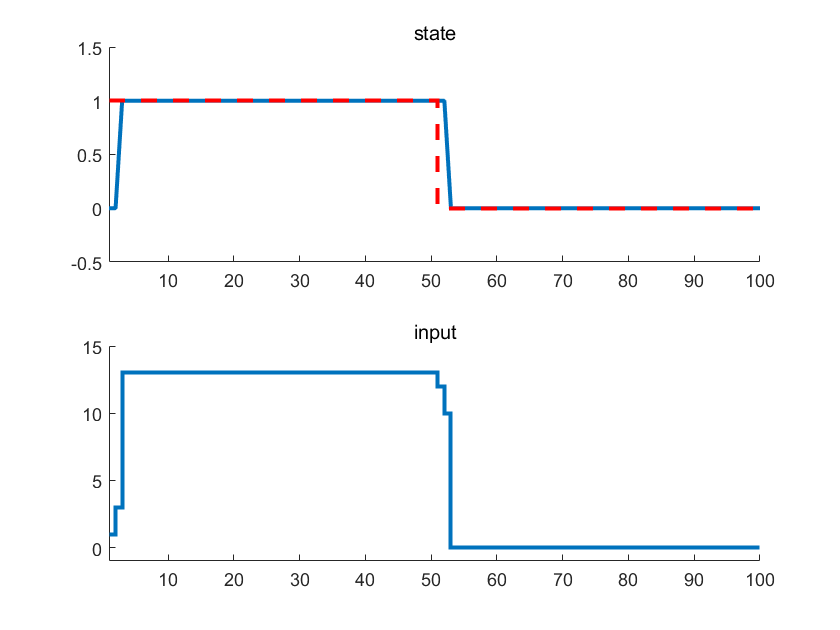
\includegraphics[width=0.7\textwidth]{pb1 0.png}
    \caption{Graph q1}\label{fig:pb2graph1}
\end{figure}
In the figure \ref{fig:pb2graph1}, the output of the system followed the
refernce well with no overshoot and no undershoot. The maximum input is
bigger than 10, $\Delta u$ is unlimited.

\subsection{$\left| u(t)\right| \leq 10, T_s=0.1s$}

\begin{figure}[h!]
    \centering
    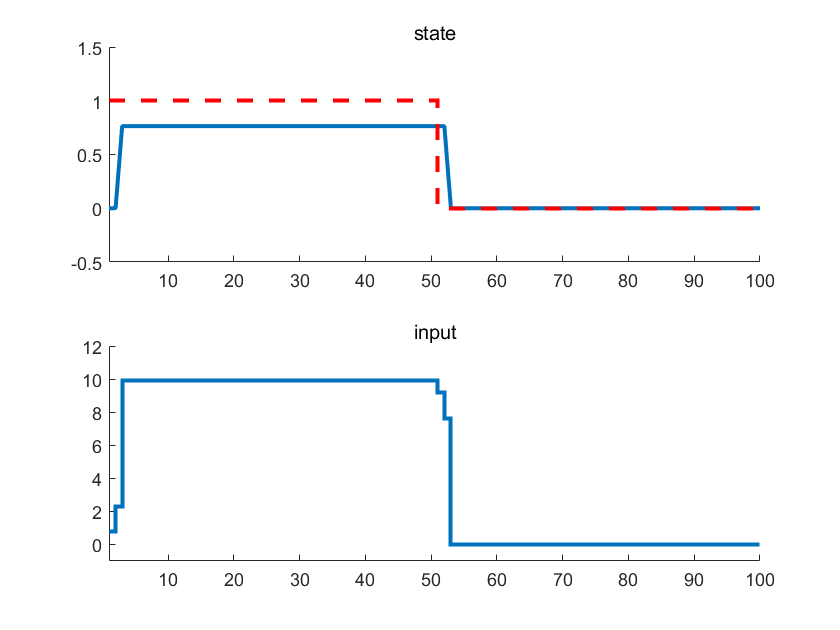
\includegraphics[width=0.7\textwidth]{pb1 1.png}
    \caption{Graph q2}\label{fig:pb2graph2}
\end{figure}
In the figure \ref{fig:pb2graph2}, the input signal is limited to 10,
the output of the system cannot follow the reference well.

\subsection{$\left| u(t)\right| \leq 10, \left| \Delta u(t) \right| \leq 1$, $T_s=0.1s$}
\begin{figure}[h!]
    \centering
    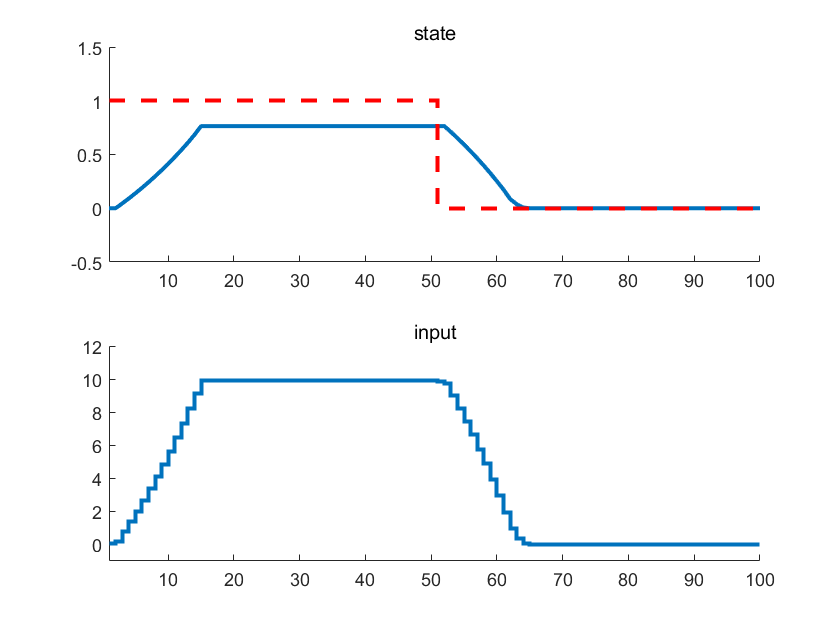
\includegraphics[width=0.7\textwidth]{pb1 2.png}
    \caption{Graph q3}\label{fig:pb2graph3}
\end{figure}
In the figure \ref{fig:pb2graph3}, the input signal is limited to 10,
and $\Delta u$ is limited to 1, the output of the system cannot follow
the reference well.

\subsection{$\left| u(t)\right| \leq 10, \left| \Delta u(t) \right| \leq 3$, $T_s=0.1s$}

\begin{figure}[h!]
    \centering
    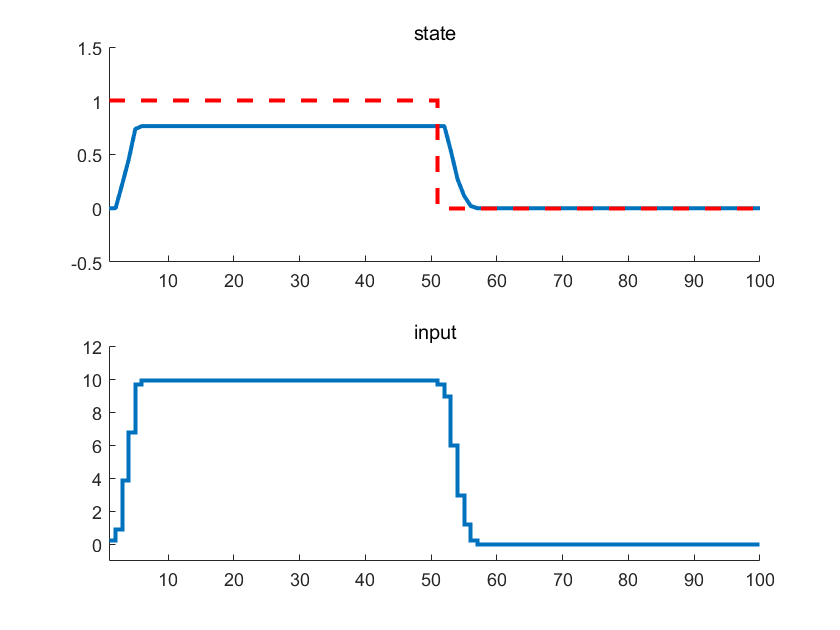
\includegraphics[width=0.7\textwidth]{pb1 3.png}
    \caption{Graph q4}\label{fig:pb2graph4}
\end{figure}
In the figure \ref{fig:pb2graph4}, the input signal is limited to 10,
and $\Delta u$ is limited to 3, the output of the system cannot follow
the reference well.

\subsection{$\left| u(t)\right| \leq 10, \left| \Delta u(t) \right| \leq 3$, $T_s=1s$}

\begin{figure}[h!]
    \centering
    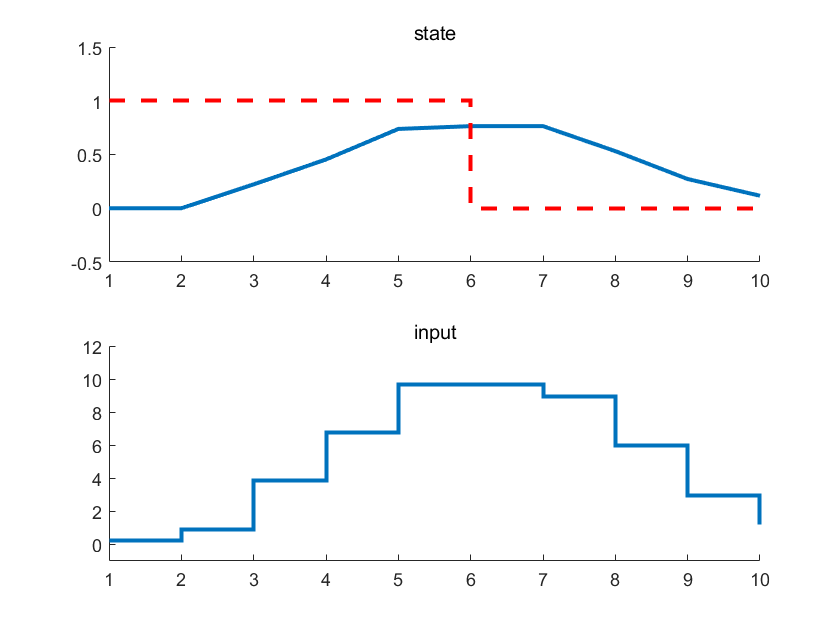
\includegraphics[width=0.7\textwidth]{pb1 4.png}
    \caption{Graph q5}\label{fig:pb2graph5}
\end{figure}
In the figure \ref{fig:pb2graph5}, the input signal is limited to 10,
and $\Delta u$ is limited to 3, the system baddly followed the reference.

\newpage
\section{Problem 3}
% insert 4 pictures here with caption
\begin{figure}[h!]
    \centering
    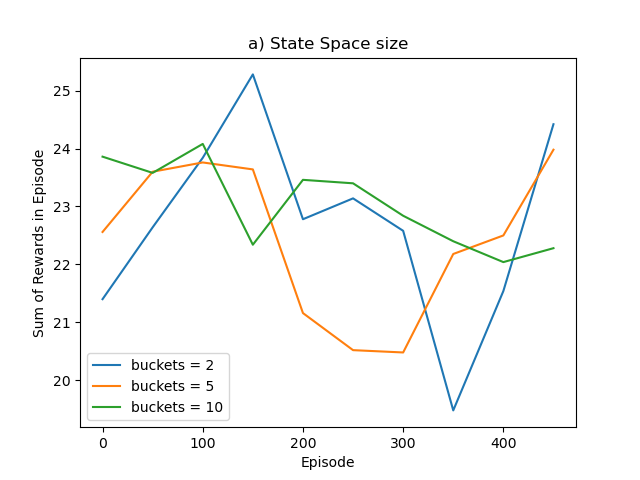
\includegraphics[width=0.7\textwidth]{graph a.png}
    \caption{Graph q1}\label{fig:pb3graph1}
\end{figure}
In the figure \ref{fig:pb3graph1}, the reward of the system is ascending,
the reward of the system is ascending. In the last episode the reward of
the system with bukets 5 is higher than the reward of the system with
bukets 10 and 2.

\begin{figure}[h!]
    \centering
    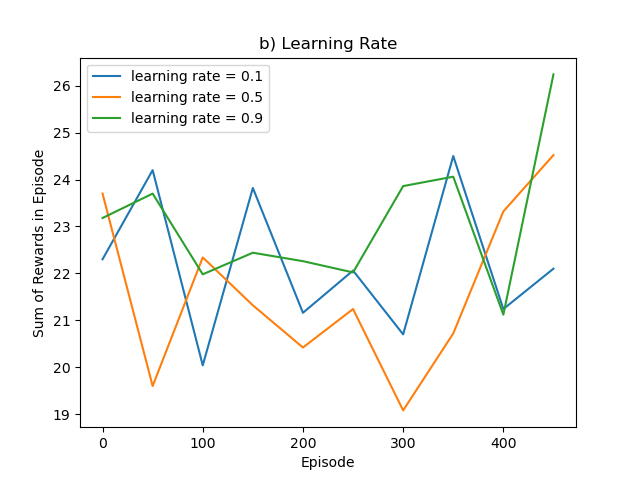
\includegraphics[width=0.7\textwidth]{graph b.png}
    \caption{Graph q2}\label{fig:pb3graph2}
\end{figure}
In the figure \ref{fig:pb3graph2}, the reward of the system is ascending,
the system with learnig rate 0.5 and 0.1 is ascending faster than the system with
learning rate 0.9.

\begin{figure}[h!]
    \centering
    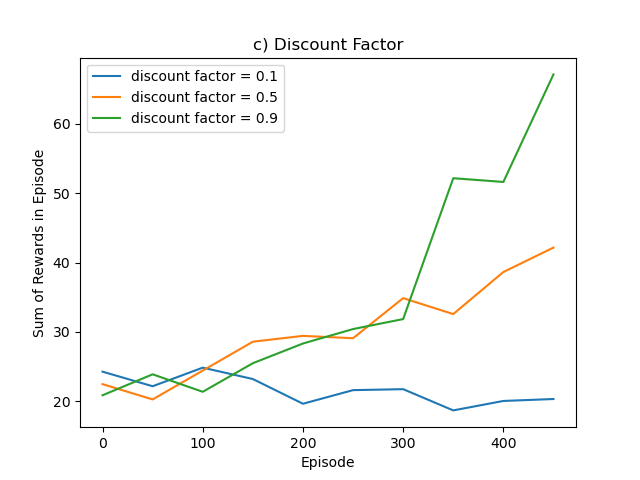
\includegraphics[width=0.7\textwidth]{graph c.png}
    \caption{Graph q3}\label{fig:pb3graph3}
\end{figure}
In the figure \ref{fig:pb3graph3}, the reward of the system is fluxuating and slightly ascending,
the performances of the system with different discout factor are similar.

\begin{figure}[h!]
    \centering
    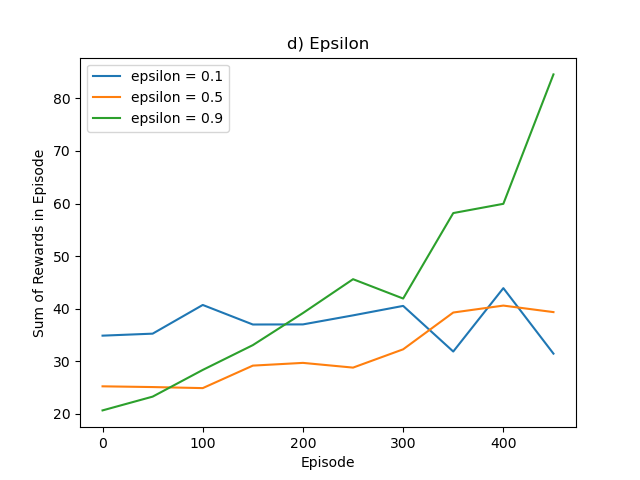
\includegraphics[width=0.7\textwidth]{graph d.png}
    \caption{Graph q4}\label{fig:pb3graph4}
\end{figure}
In the figure \ref{fig:pb3graph4}, the reward of the system is ascending,
the system with epsilon 0.1 is ascending faster than the system with epsilon 0.9.

\end{document}